\begin{figure}[ht]
    \centering
    %\begin{subfigure}[0.3\textwidth]
    \subfigure[$T>\frac{\alpha^{\prime}}{2R}$]
    {
        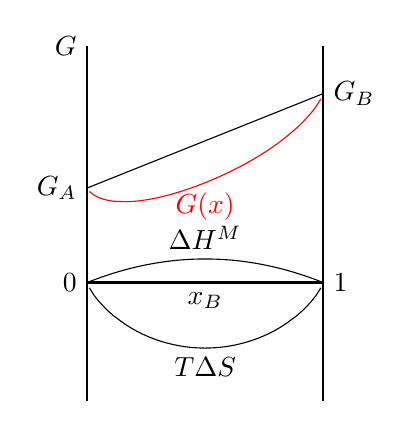
\begin{tikzpicture}[scale=3]
            \draw[thick] (0,0) node[anchor=east]{0} --(0.5,0) node[anchor=north] {$x_B$}--(1,0) node[anchor=west]{1};
            \draw[thick] (0,-0.5) -- (0,0.4) node[anchor=east]{$G_A$}--(0,1) node[anchor=east]{$G$};
            \draw[thick] (1,-0.5) -- (1,0.8) node[anchor=west]{$G_B$}--(1,1);
            
            \draw[thin] (0,0.4)--(1,0.8);
            \draw[domain=0.01:0.5] plot(\x,{0.4*(\x*ln(\x)+(1-\x)*ln((1-\x)))})
                node[below] {$T\Delta S$};
            \draw[domain=0.5:0.99] plot(\x,{0.4*(\x*ln(\x)+(1-\x)*ln((1-\x)))});
            
            %\Delta H
            \draw[domain=0:0.5] plot(\x,{0.4*(\x*(1-\x))})
                node[anchor=south] {$\Delta H^M$};
            \draw[domain=0.5:1] plot(\x,{0.4*(\x*(1-\x))});
            
            %G(x)
            \draw[red,domain=0.01:0.5] plot(\x,{0.4*\x+0.4+0.4*(\x*(1-\x))+0.4*(\x*ln(\x)+(1-\x)*ln((1-\x)))})
                node[below] {$G(x)$};
            \draw[red,domain=0.5:0.99] plot(\x,{0.4*\x+0.4+0.4*(\x*(1-\x))+0.4*(\x*ln(\x)+(1-\x)*ln((1-\x)))});        
        \end{tikzpicture}
       % \caption{$\Delta H^M=0$,混合时结合能不变的自由能曲线。}
        \label{subfig:高温下混合时结合能增加的自由能曲线}
    }
   % \end{subfigure}
   % \begin{subfigure}[0.3\textwidth]
    \subfigure[$0<T<\frac{\alpha^{\prime}}{2R}$]
    {
           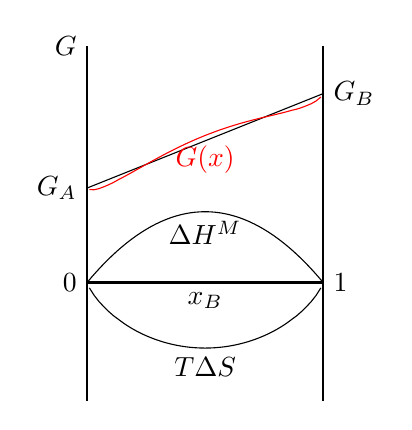
\begin{tikzpicture}[scale=3]
            \draw[thick] (0,0) node[anchor=east]{0} --(0.5,0) node[anchor=north] {$x_B$}--(1,0) node[anchor=west]{1};
            \draw[thick] (0,-0.5) -- (0,0.4) node[anchor=east]{$G_A$}--(0,1) node[anchor=east]{$G$};
            \draw[thick] (1,-0.5) -- (1,0.8) node[anchor=west]{$G_B$}--(1,1);
            %G(0)
            \draw[thin] (0,0.4)--(1,0.8);
            %T\Delta S
            \draw[domain=0.01:0.5] plot(\x,{0.4*(\x*ln(\x)+(1-\x)*ln((1-\x)))})
                node[below] {$T\Delta S$};
            \draw[domain=0.5:0.99] plot(\x,{0.4*(\x*ln(\x)+(1-\x)*ln((1-\x)))});
            %\Delta H
            \draw[domain=0:0.5] plot(\x,{1.2*(\x*(1-\x))})
                node[below] {$\Delta H^M$};
            \draw[domain=0.5:1] plot(\x,{1.2*(\x*(1-\x))});
            
            %G(x)
            \draw[red,domain=0.01:0.5] plot(\x,{0.4*\x+0.4+1.2*(\x*(1-\x))+0.4*(\x*ln(\x)+(1-\x)*ln((1-\x)))})
                node[below] {$G(x)$};
            \draw[red,domain=0.5:0.99] plot(\x,{0.4*\x+0.4+1.2*(\x*(1-\x))+0.4*(\x*ln(\x)+(1-\x)*ln((1-\x)))});        
        \end{tikzpicture}
        %\caption{$\Delta H^M<0$,混合时结合能小于零的自由能曲线。}
        \label{subfig:低温下混合时结合能增加的自由能曲线}
    }
    \subfigure[$T=0$]
    {
        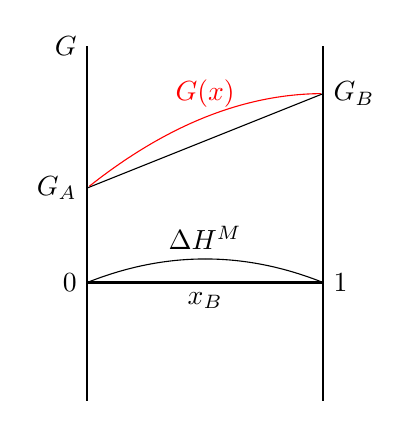
\begin{tikzpicture}[scale=3]
            \draw[thick] (0,0) node[anchor=east]{0} --(0.5,0) node[anchor=north] {$x_B$}--(1,0) node[anchor=west]{1};
            \draw[thick] (0,-0.5) -- (0,0.4) node[anchor=east]{$G_A$}--(0,1) node[anchor=east]{$G$};
            \draw[thick] (1,-0.5) -- (1,0.8) node[anchor=west]{$G_B$}--(1,1);
            %G(0)
            \draw[thin] (0,0.4)--(1,0.8);
            %T\Delta S
            %\draw[domain=0.01:0.5] plot(\x,{0.4*(\x*ln(\x)+(1-\x)*ln((1-\x)))})
            %    node[below] {$T\Delta S$};
            %\draw[domain=0.5:0.99] plot(\x,{0.4*(\x*ln(\x)+(1-\x)*ln((1-\x)))});
            %\Delta H
            \draw[domain=0:0.5] plot(\x,{0.4*(\x*(1-\x))})
                node[anchor=south] {$\Delta H^M$};
            \draw[domain=0.5:1] plot(\x,{0.4*(\x*(1-\x))});
            
            %G(x)
            \draw[red,domain=0.01:0.5] plot(\x,{0.4*\x+0.4+0.4*(\x*(1-\x))})
                node[anchor=south] {$G(x)$};
            \draw[red,domain=0.5:0.99] plot(\x,{0.4*\x+0.4+0.4*(\x*(1-\x))});        
        \end{tikzpicture}
        %\caption{$\Delta H^M<0$,混合时结合能小于零的自由能曲线。}
        \label{subfig:绝对零度下混合时结合能增加的自由能曲线}
    }
    %\end{subfigure}
    \caption{混合时结合能增加的在不同温度下的自由能曲线}

\end{figure}
